%%%%%%%%%%%%%%%%%%%%%%%%%%%%%%%%%%%%%%%%%
\documentclass[paper=a4, fontsize=15pt]{article} % A4 paper and 11pt font size

\usepackage{amsmath,amsfonts,amsthm} % Math packages
\usepackage{graphicx}
\usepackage[top=0.5in, bottom=1in, left=1in, right=1in]{geometry}
\usepackage{tabularx}


\pagestyle{plain} % Makes all pages in the document conform to the custom headers and footers

\title{	
Machine Learning \\
Homework 2
}
\author{Yao Song\\301266041} % Your name
\date{\normalsize\today} % Today's date or a custom date

\begin{document}
\maketitle % Print the title
%----------------------------------------------------------------------------------------
%	PROBLEM 1
%----------------------------------------------------------------------------------------

\section*{Question 1}
\begin{enumerate}
  \item At the green point, $p(C_1|x) = p(C_2|x) = p(C_3|x) = 1/3$
  \item When on the red line, two probabilities are equal to each other and they are bigger than the rest one.
        As an example, if it is on the red line between region 1 and region 2, then $p(C_1|x) = p(C_2|x) > p(C_3|x)$.\\
        If we move along the red line, away from the green point, two probabilities will be equally increased and remain equal, the rest one will be decreased.
        As an example, if we move along the line between region 1 and region 2, we have $p(C_1|x) = p(C_2|x)$, and both $p(C_1|x)$ and $p(C_2|x)$ will increase, $p(C_3|x)$ will decrease.
        
  \item If we move far away from the intersection point in the middle of one region, the probability of that region will increase, but the other two probabilities will both decrease .
\end{enumerate}
%%%%%%%%%%%%%%%%%%%%%%%%%%%%%%%%%%%%%%%%%%%%%%%%%%%%%%%%%%%%%%%%%%%%%%%%%%%%%%%%%%

\section*{Question 2}
The exponential kernel can be written as a power series as follows:
\begin{align*}
&\exp(k_1(x,x')) 
 = 1 + k_1(x,x') + \frac{1}{2}k^2_1(x,x') + \frac{1}{6}k^3_1(x,x') + \ldots\\
& = \sum_{d = 0}^\infty \frac{1}{d!} k_1^d(x,x') 
 = \sum_{d = 0}^\infty a_d k_1^d(x,x'), \qquad \text{where} \qquad a_d = \frac{1}{d!}.
\end{align*}
From the above equation, we can observe that the exponential kernel is a summation of infinite number of polynomial kernels.According to Eqn.6.15, for any polynomial 
$q(k_1(x,x')) = a_d k_1^d(x,x')$, there exists a feature space $\phi_d(x)$ such that 
\begin{align*}
a_d k_1^d(x,x') = \phi_d(x)^T\phi_d(x')
\end{align*}
Thus, we get the following equation:
\begin{align*}
\exp(k_1(x,x')) = \sum_{d = 0}^\infty \phi_d(x)^T\phi_d(x').
\end{align*}
As a result, the infinite dimensional space of $\exp(k_1(x,x')) $ can be written as
$\exp(k_1(x,x'))  = \phi_{inf}(x)^T\phi_{inf}(x')$, 
where $\phi_{inf}(x) = \begin{pmatrix} \phi_{0}(x)\\ \phi_{1}(x)\\ \phi_{2}(x)\\ \ldots \end{pmatrix}$
 is a infinite dimensional column vector.
%%%%%%%%%%%%%%%%%%%%%%%%%%%%%%%%%%%%%%%%%%%%%%%%%%%%%%%%%%%%%%%%%%%%%%%%%%%%%%%%%%



\section*{Question 3}
The corresponding Langrangian is given by
\begin{align*}
L(w,b,\epsilon, a) = \frac{1}{2}\lVert{w}\rVert^2 +  C_1 \sum_{n \in N}{\epsilon_n}
+ C_2 \sum_{n \in P}{\epsilon_n}
- \sum_n a_n (t_n y(x_n) -1 + \epsilon_n)
- \sum_n \mu_n \epsilon_n,
\end{align*}
where $a_n \geq 0$ and $\mu_n \geq 0$ are langrangian multipliers.\\
The KKT conditions are listed as follows:
\begin{align*}
\epsilon_n \geq 0,  \qquad \forall n\\
a_n \geq 0, \qquad \forall n\\
\mu_n  \geq 0, \qquad \forall n\\
t_n y(x_n) -1 + \epsilon_n \geq 0, \qquad \forall n\\
a_n (t_n y(x_n) -1 + \epsilon_n) = 0, \qquad \forall n \\
\mu_n \epsilon_n = 0, \qquad \forall n
\end{align*}
Let us take derivative of the Langrangian over $w,b,\epsilon_n$ separately.
\begin{align*}
& \frac{\partial L}{\partial w} = 0  \xrightarrow[]{ } w = \sum_n a_n t_n \phi(x_n) \\
&  \frac{\partial L}{\partial b} = 0  \xrightarrow[]{ } \sum_n a_n t_n = 0 \\
&   \frac{\partial L}{\partial \epsilon_n} = 0  \xrightarrow[]{ }
a_n = C_1 - \mu_n, \forall n \in P, \qquad
a_n = C_2 - \mu_n,  \forall n \in N
\end{align*}
By using the above results, we can remove $w,b,\epsilon_n$ from the Langrangian and get the dual form Langrangian
\begin{align*}
\tilde{L}(a) = \sum_n a_n - \frac{1}{2}\sum_n \sum_m a_n a_m t_n t_m k(x_n,x_m)
\end{align*}
And the box constraints are 
\begin{align*}
& 0 \leq a_n \leq C_1, \qquad \forall n \in P\\
& 0 \leq a_n \leq C_2, \qquad \forall n \in N \\
& \sum_n a_n t_n = 0
\end{align*}
%%%%%%%%%%%%%%%%%%%%%%%%%%%%%%%%%%%%%%%%%%%%%%%%%%%%%%%%%%%%%%%%%%%%%%%%%%%%%%%%%%



\section*{Question 4}

\begin{enumerate}
\item The plots are oscillating because the step size is too large. When the step size is large, each time we will jump around the optimal point, but not directly to the optimal point. If the step size is larger, this figure will show a larger oscillation.
The results are shown in Fig. \ref{fig:sg2} and Fig. \ref{fig:sg3}\\
We can fix this oscillation problem by setting a smaller step size with care. Now we will go straightforward to the optimal point direction. 
Note some step size values will not lead to the optimal point, but break the iteration loop early, that is not what we want.
We choose the step size to be $eta = 0.001$. 
Note that this eta is not the best one. There are other eta values which can achieve lower objective values. The results are shown in Fig. \ref{fig:sg2001} and Fig. \ref{fig:sg3001}.
\begin{figure}[hb]
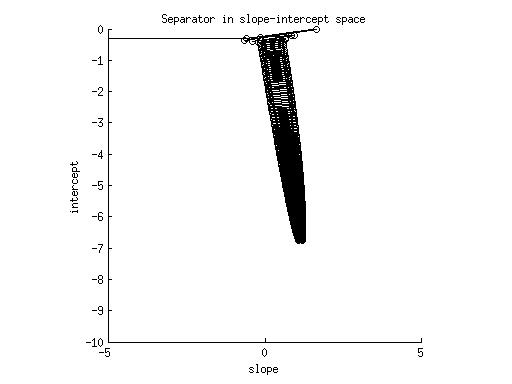
\includegraphics[width=\linewidth]{./a2_datacode/lr/fig2_gd.jpg}
\caption{separator path with eta = 0.003, obvious oscillation}
\label{fig:sg2}
\end{figure}
\begin{figure}[hb]
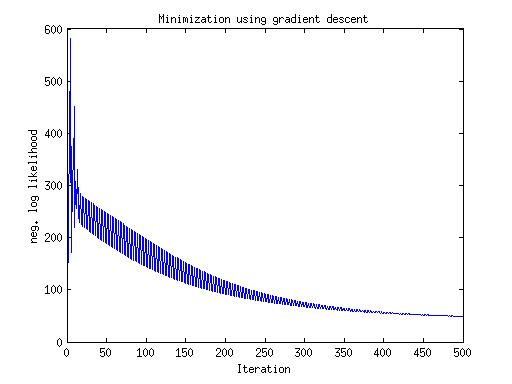
\includegraphics[width=\linewidth]{./a2_datacode/lr/fig3_gd.jpg}
\caption{neg. likelihood over iterations with eta = 0.003, obvious oscillation}
\label{fig:sg3}
\end{figure}
\begin{figure}[hb]
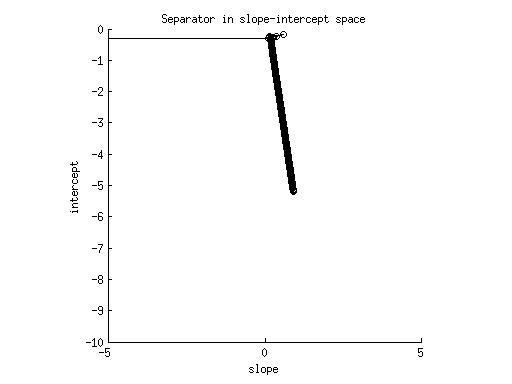
\includegraphics[width=\linewidth]{./a2_datacode/lr/fig2_gd_001.jpg}
\caption{separator path with eta = 0.001, no oscillation}
\label{fig:sg2001}
\end{figure}
\begin{figure}[hb]
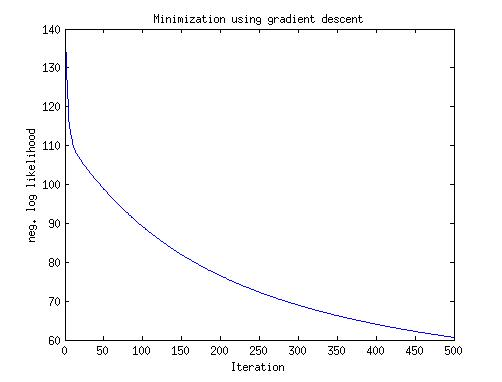
\includegraphics[width=\linewidth]{./a2_datacode/lr/fig3_gd_001.jpg}
\caption{neg. likelihood over iterations with eta = 0.001, no oscillation}
\label{fig:sg3001}
\end{figure}
%%%%%%%%%%%%%%%%%%%%%%%%%%%%%%%%%%%%%%%%%%%%%%%%%%%%%%%%%%%%%%%%%%%%%%%%%%%%%%%%%%
\item 
%In the code, the maximum iteration is changed to 2000 to get closer to the optimal point. This is because the stochastic gradient descent is slower in convergence.\\
%The stopping criteria is changed to $tol = 0.0001$ to prevent early loop break.
%This is because in stochastic gradient descent, the error differences between two iterations is much smaller than that of the batch gradient descent. The step size is not changed.
The results are shown in Fig. \ref{fig:sgtrue2} and Fig.\ref{fig:sgtrue3}
\begin{figure}[hb]
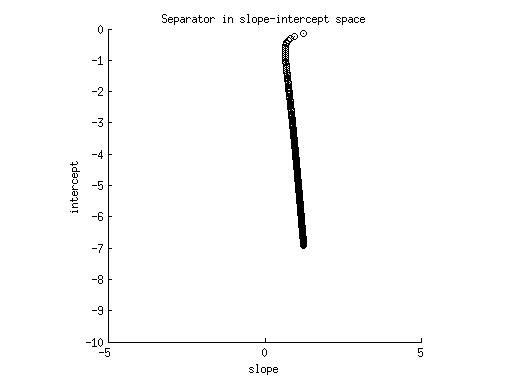
\includegraphics[width=\linewidth]{./a2_datacode/lr/fig2_sg.jpg}
\caption{separator path of stochastic gradient descent}
\label{fig:sgtrue2}
\end{figure}
\begin{figure}[hb]
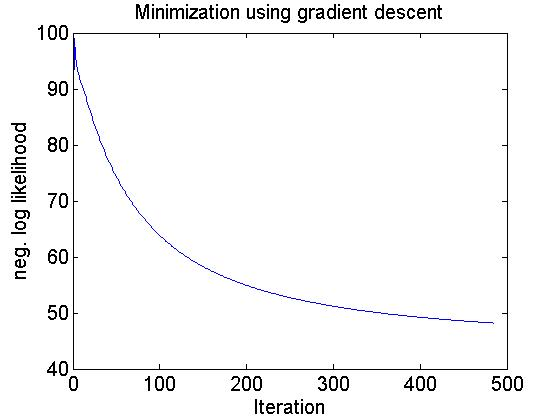
\includegraphics[width=\linewidth]{./a2_datacode/lr/fig3_sg.jpg}
\caption{neg. likelihood over iterations of stochastic gradient descent}
\label{fig:sgtrue3}
\end{figure}
%%%%%%%%%%%%%%%%%%%%%%%%%%%%%%%%%%%%%%%%%%%%%%%%%%%%%%%%%%%%%%%%%%%%%%%%%%%%%%%%%%
\item The IRLS algorithm takes only 7 iterations to reach convergence. The results form IRLS are shown in Fig.\ref{fig:irls2} and Fig.\ref{fig:irls3}.
\begin{figure}[hb]
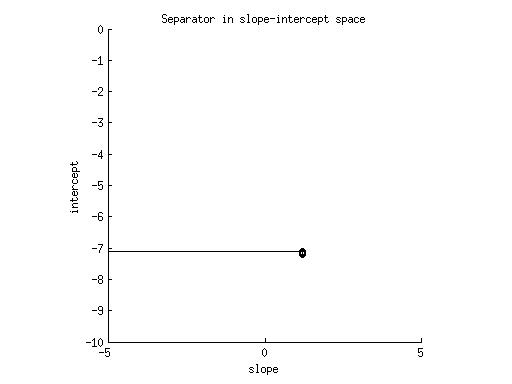
\includegraphics[width=\linewidth]{./a2_datacode/lr/fig2_irls.jpg}
\caption{separator path of IRLS}
\label{fig:irls2}
\end{figure}
\begin{figure}[hb]
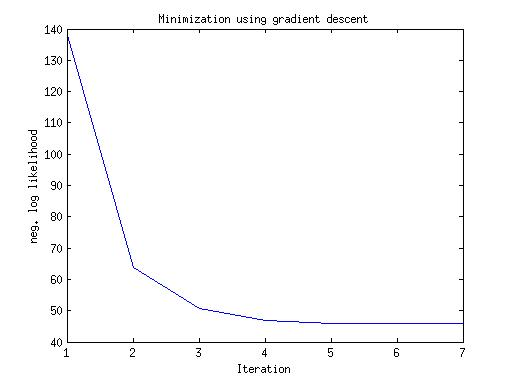
\includegraphics[width=\linewidth]{./a2_datacode/lr/fig3_irls.jpg}
\caption{neg. likelihood over iterations of IRLS}
\label{fig:irls3}
\end{figure}
\end{enumerate}
%%%%%%%%%%%%%%%%%%%%%%%%%%%%%%%%%%%%%%%%%%%%%%%%%%%%%%%%%%%%%%%%%%%%%%%%%%%%%%%%%%
\section*{Question 5}
The following figures show the cross validation results.
The tuning of C parameter for linear model is shown in Fig. \ref{fig:linear_model}.
The soft margin constant C will determine the position of the decision boundary. A large C means a large penalty for misclassified points.\\
The tuning of parameter C and $\gamma$ for the rbf kernel is shown in Fig. \ref{fig:rbf_model}. It can achieve a score above 59.
The parameter $\gamma$ is the inverse kernel width. Large value of $\gamma$ will give the model more flexibility.\\
The polynomial kernel behaves quite bad in this task.The accuracy stays at around 26.6 for various values of C and degree pairs. So the figure is not shown here.\\
The tuning of parameter C and $\gamma$ for the sigmoid kernel is shown in Fig. \ref{fig:sigmoid_model}.
It can achieve a score above 59. \\
According to the experimentation results, I decide the best classifier for this task is the linear kernel with C = 150. We can achieve an accuracy of 59.6 with these parameters and Ptest is generated by them.


\begin{figure}[hb]
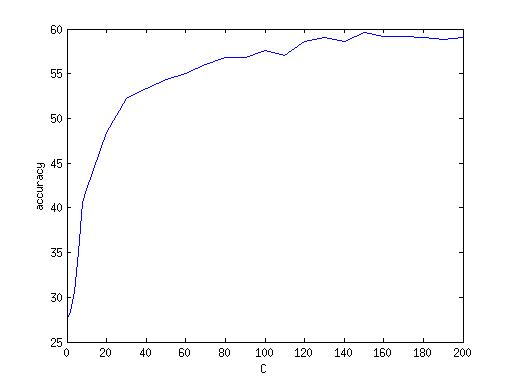
\includegraphics[width=\linewidth]{./a2_datacode/lr/linear_model_parameter.jpg}
\caption{accuracy over the parameter C for linear kernel}
\label{fig:linear_model}
\end{figure}

\begin{figure}[hb]
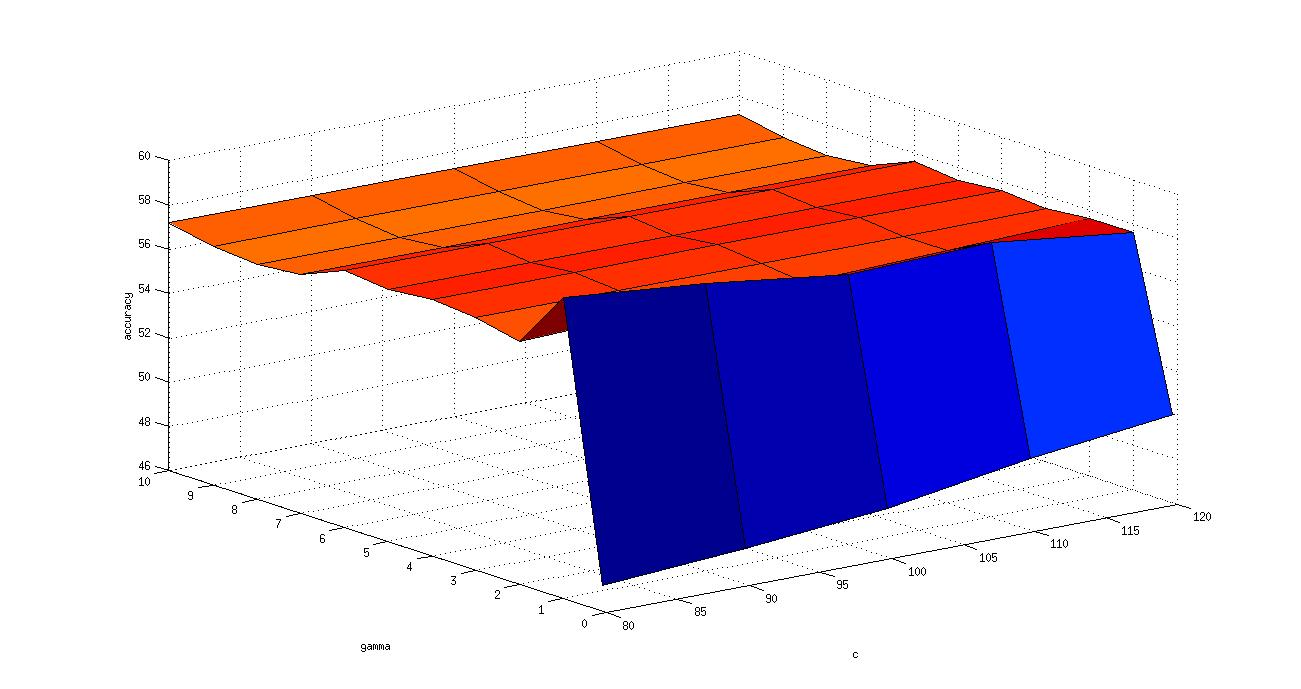
\includegraphics[width=\linewidth]{./a2_datacode/lr/rbf_parameter.jpg}
\caption{accuracy over parameter C and gamma for rbf kernel}
\label{fig:rbf_model}
\end{figure}

\begin{figure}[hb]
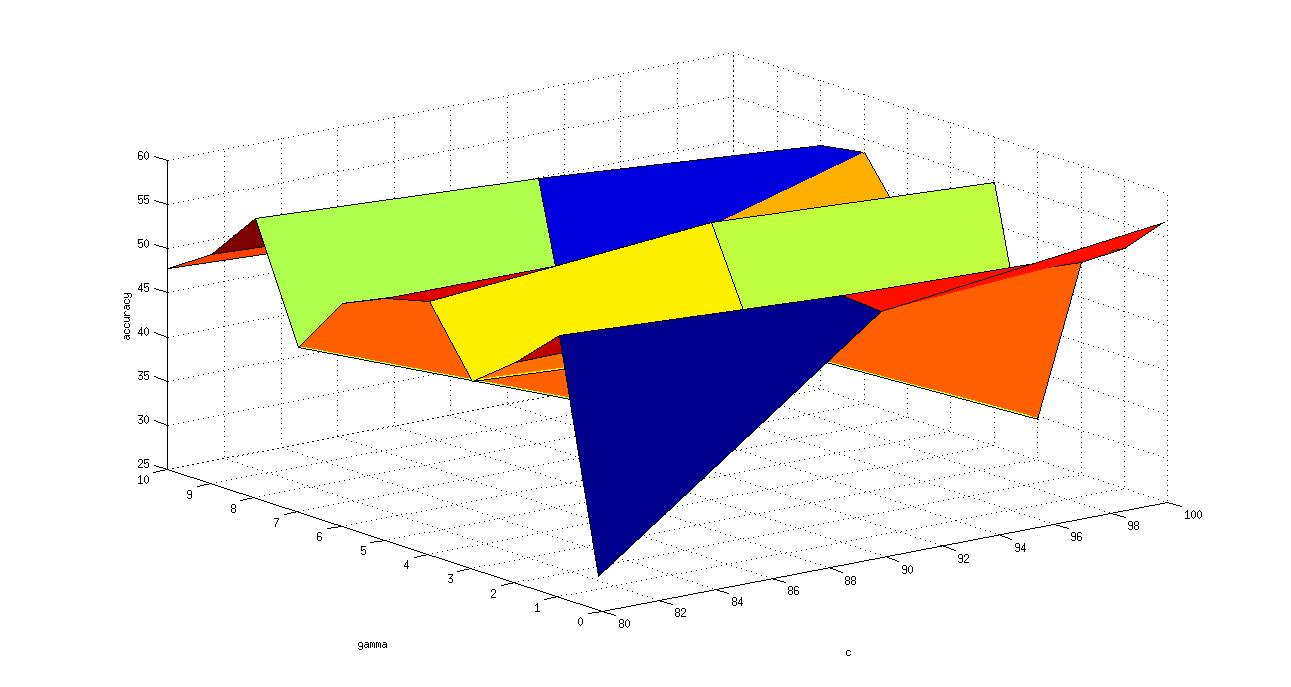
\includegraphics[width=\linewidth]{./a2_datacode/lr/sigmoid.jpg}
\caption{accuracy over parameter C and gamma for sigmoid kernel}
\label{fig:sigmoid_model}
\end{figure}
%----------------------------------------------------------------------------------------

\end{document}